\uuid{1Ozf}
\exo7id{6982}
\auteur{blanc-centi}
\datecreate{2015-07-04}
\isIndication{false}
\isCorrection{true}
\chapitre{Courbes planes}
\sousChapitre{Courbes paramétrées}

\contenu{
\texte{
\
}
\begin{enumerate}
    \item \question{Donner une paramétrisation $(x(t),y(t))$ de la courbe d'équation $$y=\sqrt{-x^2-3x+4}$$ en précisant le domaine de variation du paramètre $t$.}
\reponse{Pour transformer une équation cartésienne $y=f(x)$ en paramétrisation, il suffit de poser $x=t$ et $y=f(t)$, en faisant décrire au paramètre $t$ le domaine de définition de $f$. Ici, $f(x)=\sqrt{-x^2-3x+4}$ est bien définie pour les $x\in\R$ tels que $-x^2-3x+4\ge 0$ \textsl{i.e.} $x\in[-4;-1]$. On obtient donc la paramétrisation suivante:
$$\left\{\begin{array}{l}
x(t)=t\\
y(t)=\sqrt{-t^2-3t+4}
\end{array}\quad (t\in[-4;1])\right.$$
ce qui signifie
\begin{eqnarray*}
(x,y)\in\mathcal{C}&\Longleftrightarrow&\left\{\begin{array}{l}
x\in[-4;1]\\
y=\sqrt{-x^2-3x+4}
\end{array}\right.\\
 &\Longleftrightarrow&\exists\, t\in[-4;1]\ |\ \left\{\begin{array}{l}
x(t)=t\\
y(t)=\sqrt{-t^2-3t+4}
\end{array}\right.
\end{eqnarray*}
où $\mathcal{C}$ est la courbe étudiée.

\begin{center}
 \begin{tikzpicture}[scale=1]

     \draw[->,>=latex,thick, gray] (-4.5,0)--(2,0) node[below,black] {$x$};
     \draw[->,>=latex,thick, gray] (0,-1)--(0,6) node[right,black] {$y$};  


  \draw[red, very thick,domain=-4:1,samples=100] plot ({\x},{sqrt(-\x*\x-3*\x+4))}) ;
  
  \node[black, above right] at (-4,5.6) {$y=\sqrt{-x^2-3x+4}$};


  \draw[blue, dashed] (-4,0)--(-4,5.6); 
  \fill[blue] (-4,0) circle (2pt)  node[below]{$-4$}; 

 
  \fill[blue] (1,0) circle (2pt)  node[below]{$1$}; 
\end{tikzpicture} 
\end{center}}
    \item \question{Montrer que le support de la courbe paramétrée par
$$\left\{\begin{array}{l}x(t)=\cos t +3\\ y(t)=\sin t\end{array}\quad(t\in\R)\right.$$
ne peut pas \^etre décrit par une équation de la forme $y=f(x)$.}
\reponse{S'il est toujours possible de représenter le graphe d'une fonction comme une courbe 
paramétrée, la réciproque n'est pas vraie. Ici, la courbe considérée est le cercle de 
rayon $1$ centré au point $(3,0)$. Ce n'est donc pas un graphe de fonction, puisque 
plusieurs points de la courbe ont la m\^eme abscisse: conna\^itre $x$ ne donne pas 
$y$! Par exemple, pour $t=\pm\frac{\pi}{2}$, on obtient les deux points de la courbe $(3,-1)$ et $(3,+1)$.
\begin{center}
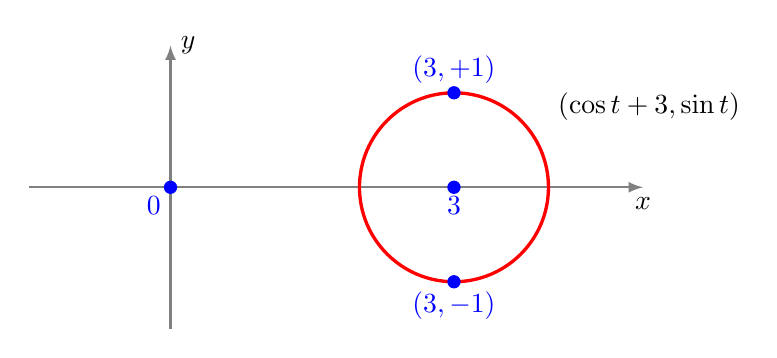
\begin{tikzpicture}[scale=1.2]

     \draw[->,>=latex,thick, gray] (-1.5,0)--(5,0) node[below,black] {$x$};
     \draw[->,>=latex,thick, gray] (0,-1.5)--(0,1.5) node[right,black] {$y$};  


  \draw[red, very thick,domain=-4:1,samples=100] (3,0) circle (1cm);
  \node[black, above right] at (4,0.6) {$(\cos t + 3,\sin t)$};

  \fill[blue] (0,0) circle (2pt) node[below left]{$0$}; 
  \fill[blue] (3,0) circle (2pt)  node[below]{$3$}; 
  
  \fill[blue] (3,1) circle (2pt)  node[above]{$(3,+1)$}; 
  \fill[blue] (3,-1) circle (2pt)  node[below]{$(3,-1)$};   
\end{tikzpicture}  
\end{center}}
    \item \question{Montrer que le support de la courbe paramétrée par
$$\left\{\begin{array}{l}x(t)=\cos^2t-2\\ y(t)=\sin^4t+4\sin^2t+4\end{array}\quad(t\in\R)\right.$$
est le graphe d'une fonction $f$ que l'on précisera, ainsi que son domaine de définition.}
\reponse{On constate, en utilisant la formule $\sin^2t=1-\cos^2t=-1-x(t)$, que
\begin{eqnarray*}
y(t)&=&\sin^4t+4\sin^2t+4=(-1-x(t))^2+4(-1-x(t))+4\\
 &=&x(t)^2-2x(t)+1 = (x(t)-1)^2
\end{eqnarray*}
Ainsi les points $(x,y)$ de la courbe vérifient l'équation $y=(x-1)^2$. 
De plus, lorsque le paramètre $t$ décrit $\R$, $x(t)=\cos^2t-2$ décrit l'intervalle $[-2;-1]$. Finalement, 
\begin{eqnarray*}
(x,y)\in\mathcal{C}&\Longleftrightarrow&\exists\, t\in\R\ |\ \left\{\begin{array}{l}
x(t)=\cos^2t-2\\
y(t)=\sin^4t+4\sin^2t+4
\end{array}\right.\\
\ &\Longleftrightarrow&\left\{\begin{array}{l}
x\in[-2;-1]\\
y=(x-1)^2
\end{array}\right.
\end{eqnarray*}
et la courbe est donc le graphe de la fonction
$$\begin{array}{rccc}
f:&[-2;-1]&\to&\R\\
\ &x&\mapsto&(x-1)^2
\end{array}$$

\begin{center}
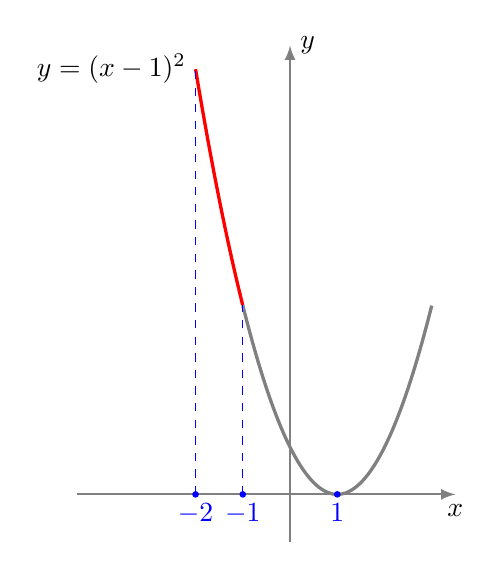
\begin{tikzpicture}[scale=0.6]

     \draw[->,>=latex,thick, gray] (-4.5,0)--(3.5,0) node[below,black] {$x$};
     \draw[->,>=latex,thick, gray] (0,-1)--(0,9.5) node[right,black] {$y$};  


  \draw[red, very thick,domain=-2:-1,samples=100] plot ({\x},{(\x-1)*(\x-1)}) ;
  \draw[gray, very thick,domain=-1:3,samples=100] plot ({\x},{(\x-1)*(\x-1)}) ;  
  \node[black, left] at (-2,9) {$y=(x-1)^2$};


  \draw[blue, dashed] (-2,0)--(-2,9); 
  \fill[blue] (-2,0) circle (2pt)  node[below]{$-2$}; 
  \draw[blue, dashed] (-1,0)--(-1,4); 
  \fill[blue] (-1,0) circle (2pt)  node[below]{$-1$};
 
  \fill[blue] (1,0) circle (2pt)  node[below]{$1$}; 
\end{tikzpicture}
\end{center}}
\end{enumerate}
}
